\chapter{Algorithm}
\section{Score-based Diffusion Model}
Before diffusion models were introduced, generative models were primarily based on Variational Autoencoders (VAEs) and Generative Adversarial Networks (GANs). While VAEs are effective for compressing data, they struggle to generate high-quality, diverse samples due to their reliance on sampling from a normal distribution in the latent space. GANs, on the other hand, have demonstrated success in generating realistic samples but can be challenging to train and prone to mode collapse.

One drawback of Variational Autoencoders (VAEs) is the inclusion of the KL divergence term in their loss function. While VAEs are effective for compressing data (encoding), they struggle to generate high-quality, diverse samples. This limitation stems from their reliance on sampling from a normal distribution in the latent space. Although VAEs are trained to bring the posterior distribution close to a Gaussian, in practice, the match is often not precise enough to ensure that samples drawn from this distribution will be of high quality.

Therefore, an alternative approach, introduced in 2015, is the “diffusion model,” which can be implemented using either score-matching or denoising techniques. Diffusion models aim to generate synthetic data based on a set of independent, identically distributed (i.i.d.) samples drawn from an unknown data distribution. The key concept is to simulate new samples by either employing denoising Score Langevin Dynamics (SMLD) or implementing Denoising Diffusion Probabilistic Model (DDPM), where a deep neural network approximates the score, or gradient, of the log-density of the data distribution. Next we will discuss the two methods in detail.

\subsection{Denoising Score Matching with Langevin Dynamics (SMLD)}
Langevin Dynamics in generative modeling is a way to generate samples by simulating a process that gradually moves from random points in space toward areas with high probability density, where most of the real data is located. It does this by changing along the directions defined by the gradient of the probability distribution, called the "score" in our context. At each step, a small amount of Gaussian noise is added to introduce randomness, ensuring that each path taken is unique and prevents the sampling process from getting "stuck" in local regions.

In simpler terms, think of Langevin Dynamics as a guided walk starting from a random spot and following a path that gradually leads toward more typical or likely values of the data (like images, text, etc.). The direction of each step is influenced by both the data structure (moving toward areas where data is dense) and a bit of noise to keep things varied, which helps to explore the whole space more effectively. This makes Langevin Dynamics an effective sampling method for creating new data points in generative modeling.

In this approach, we define a perturbation mechanism \( p_\sigma(\tilde{x} | x) = \mathcal{N}(\tilde{x}; x, \sigma^2 I) \), which acts as a Gaussian kernel centered at \( x \) with variance \( \sigma^2 \). This perturbation is integrated over the data distribution \( p_{\text{data}}(x) \) to yield the broader distribution \( p_\sigma(\tilde{x}) = \int p_{\text{data}}(x) p_\sigma(\tilde{x} | x) \, dx \). 

We consider a range of increasing noise scales, where \( \sigma_{\min} = \sigma_1 < \sigma_2 < \dots < \sigma_N = \sigma_{\max} \). Typically, \( \sigma_{\min} \) is chosen to be small enough that \( p_{\sigma_{\min}}(x) \approx p_{\text{data}}(x) \), capturing the original data distribution, while \( \sigma_{\max} \) is set large enough so that \( p_{\sigma_{\max}}(x) \approx \mathcal{N}(x; 0, \sigma_{\max}^2 I) \), resembling a Gaussian prior.

Following the work of Song and Ermon \cite{song_generative_2020}, we train a Noise Conditional Score Network (NCSN), denoted \( s_\theta(x, \sigma) \), by minimizing a weighted sum of denoising score matching objectives as follows:

\begin{equation}
\theta^* = \arg \min_{\theta} \sum_{i=1}^{N} \sigma_i^2 \, \mathbb{E}_{p_{\text{data}}(x)} \, \mathbb{E}_{p_{\sigma_i}(\tilde{x} | x)} \left[ \| s_\theta(\tilde{x}, \sigma_i) - \nabla_{\tilde{x}} \log p_{\sigma_i}(\tilde{x} | x) \|_2^2 \right].
\end{equation}

Given sufficient data and model capacity, the resulting score-based model \( s_\theta^*(x, \sigma) \) estimates the gradient \( \nabla_x \log p_{\sigma}(x) \) across noise scales \( \sigma \in \{\sigma_i\}_{i=1}^{N} \).

So the Langevin Dynamics process can be described as follows:

\begin{equation}
\mathbf{x}_i = \mathbf{x}_{i-1} + \sqrt{\sigma_{i}^2 - \sigma_{i-1}^2} \mathbf{z}_{i-1} , i = 1, 2, \dots, N
\end{equation}



\subsection{ Denoising Diffusion Probabilistic Model (DDPM)}
Next, we are going to introduce the second method for diffusing models, the Denoising Diffusion Probabilistic Model (DDPM)~\cite{DDPM_2020}. Unlike SMLD, DDPM incorporates a scaling factor for \( x \), which modifies the approach slightly. The basic idea is to define the conditional probability distribution as follows: \( p(x_i | x_{i-1}) = \mathcal{N} \left( x_i ; \sqrt{1 - \beta_i} x_{i-1}, \beta_i I \right) \).

Following Sohl-Dickstein et al.~\cite{Dickstein2015} and Ho et al.~\cite{DDPM_2020}, let us consider a set of positive noise scales \( 0 < \beta_1, \beta_2, \dots, \beta_N < 1 \). For each data point \( x_0 \sim p_{\text{data}}(x) \), we define a discrete Markov chain \( \{x_0, x_1, \dots, x_N\} \), with each transition given by \( p(x_i | x_{i-1}) = \mathcal{N} \left( x_i ; \sqrt{1 - \beta_i} x_{i-1}, \beta_i I \right) \). Consequently, we can write the marginal distribution \( p_{\alpha_i}(x_i | x_0) = \mathcal{N} \left( x_i ; \sqrt{\alpha_i} x_0, (1 - \alpha_i) I \right) \), where \( \alpha_i := \prod_{j=1}^i (1 - \beta_j) \).

As in SMLD, we also train it by minimizing the denoising score matching objective:

\begin{equation}
\theta^* = \arg \min_{\theta} \sum_{i=1}^{N} (1-\alpha_i) \, \mathbb{E}_{p_{\text{data}}(x)} \, \mathbb{E}_{p_{\alpha_i}(\tilde{x} | x)} \left[ \| s_\theta(\tilde{x}, \alpha_i) - \nabla_{\tilde{x}} \log p_{\alpha_i}(\tilde{x} | x) \|_2^2 \right].
\end{equation}

where again, $1-\alpha_i$ is just a weighting factor.

What's more, we can define the perturbed data distribution as \( p_{\alpha_i}(\tilde{x}) := \int p_{\text{data}}(x) p_{\alpha_i}(\tilde{x} | x) dx \). The noise scales are chosen so that \( x_N \) approximates a standard normal distribution \( \mathcal{N}(0, I) \). So the simialr form as SMLD will be 

\begin{equation}
    x_{t-1} = \sqrt{1 - \beta_t} x_t + \sqrt{\beta_t} z_t, \quad t = N, N-1, \dots, 1  
\end{equation}

where \( z_t \sim \mathcal{N}(0, I) \) are standard normal samples. The final sample \( x_0 \) is drawn from the data distribution \( p_{\text{data}}(x) \). The process is repeated for each data point, and the final samples are generated by running the Markov chain for \( T \) steps. The resulting samples are expected to approximate the data distribution \( p_{\text{data}}(x) \) when \( T \to \infty \) under suitable conditions.
\section{Forward Process}
So far, we have discussed two ways of simulating new samples from a given data distribution. Although they look different, both methods are based on the same principle: iteratively transforming a sample from a simple distribution (e.g., a Gaussian) to a more complex one (e.g., the data distribution). 

Based on the work of Yang Song \cite{song_generative_2020}, we can generalize this concept through what is called the \textbf{forward process} in diffusion models.

Our goal is to construct a diffusion process \( x_{t} \) indexed by a continuous time variable \( t \in [0, T] \), such that:
\begin{equation}
    x_{0} \sim p_{0}
\end{equation}
for which we have a dataset of independent and identically distributed (i.i.d.) samples, and
\begin{equation}
    x_{T} \sim p_{T}
\end{equation}
for which we have a tractable form to generate samples efficiently. In other words, \( p_{0} \) is the data distribution and \( p_{T} \) is the prior distribution.

This diffusion process can be modeled as the solution to an Itô stochastic differential equation (SDE):
\begin{equation}
    dx = f(x, t) \, dt + g(t) \, dw
\end{equation}
where:
\begin{itemize}
    \item \( x \) is the state variable,
    \item \( f(x, t) \) is the drift coefficient,
    \item \( g(t) \) is the diffusion coefficient,
    \item \( w \) is a Wiener process (Brownian motion).
\end{itemize}

For later we can show that this has a slightly better result than orginal DDPM and SMLD.



\section{Backward Process}

With the forward process established, we can now construct the \textbf{backward process}. The aim of this process is to generate samples from the data distribution \( p_{0} \), given samples from the prior distribution \( p_{T} \).

The continuous form of this process is defined by the following stochastic differential equation (SDE):

\begin{equation}
d\mathbf{x} = \mathbf{f}_t(\mathbf{x}) \, dt + g_t \, d\mathbf{w} \label{eq:sde-forward}
\end{equation}

To direclty prove the reverse SDE formula in continuous form will be a little complex. But we can get the same spirit from discrete form, as \( \Delta t \to 0 \), the continuous equation above can be approximated by:

\begin{equation}
\mathbf{x}_{t+\Delta t} - \mathbf{x}_t = \mathbf{f}_t(\mathbf{x}_t) \, \Delta t + g_t \sqrt{\Delta t} \, \mathbf{\varepsilon}, \quad \mathbf{\varepsilon} \sim \mathcal{N}(\mathbf{0}, \mathbf{I}) \label{eq:sde-discrete}
\end{equation}

The discrete form of the stochastic differential equation (SDE) is especially valuable for practical computer implementations. By breaking down the continuous process into discrete steps, we can simulate both the diffusion and reverse processes incrementally, allowing us to generate samples using numerical methods. This approach enables us to approximate continuous dynamics with a series of discrete updates, making the computations more manageable and efficient.

In this way, using the SDE framework to describe diffusion models provides a clear distinction between theoretical analysis and practical implementation. We can rely on the mathematical properties of continuous SDEs for analysis, while in actual applications, we have the flexibility to choose any appropriate discretization method for efficient numerical calculation.

In probabilistic terms, Equation \eqref{eq:sde-discrete} implies that the conditional probability is given by

\begin{equation}
\begin{aligned}
p(\mathbf{x}_{t+\Delta t}|\mathbf{x}_t) =&\, \mathcal{N}\left(\mathbf{x}_{t+\Delta t}; \mathbf{x}_t + \mathbf{f}_t(\mathbf{x}_t) \, \Delta t, g_t^2 \, \Delta t \, \mathbf{I}\right) \\
\propto&\, \exp\left(-\frac{\|\mathbf{x}_{t+\Delta t} - \mathbf{x}_t - \mathbf{f}_t(\mathbf{x}_t) \, \Delta t\|^2}{2 g_t^2 \Delta t}\right)
\end{aligned} \label{eq:sde-proba}
\end{equation}

Now since our goal is to use the forward process to derive the backward process, which means obtaining \( p(\mathbf{x}_t|\mathbf{x}_{t+\Delta t}) \), we apply Bayes' theorem, as shown in "A Discussion on Generative Diffusion Models: DDPM = Bayesian + Denoising":~\cite{noauthor_ddpm_nodate}

\begin{equation}
\begin{aligned}
p(\mathbf{x}_t|\mathbf{x}_{t+\Delta t}) =&\, \frac{p(\mathbf{x}_{t+\Delta t}|\mathbf{x}_t) p(\mathbf{x}_t)}{p(\mathbf{x}_{t+\Delta t})} \\
=&\, p(\mathbf{x}_{t+\Delta t}|\mathbf{x}_t) \exp\left(\log p(\mathbf{x}_t) - \log p(\mathbf{x}_{t+\Delta t})\right) \\
\propto&\, \exp\left(-\frac{\|\mathbf{x}_{t+\Delta t} - \mathbf{x}_t - \mathbf{f}_t(\mathbf{x}_t) \Delta t\|^2}{2 g_t^2 \Delta t} + \log p(\mathbf{x}_t) - \log p(\mathbf{x}_{t+\Delta t})\right)
\end{aligned} \label{eq:bayes-dt}
\end{equation}

It is not difficult to see that when \( \Delta t \) is sufficiently small, \( p(\mathbf{x}_{t+\Delta t}|\mathbf{x}_t) \) will be significantly non-zero only when \( \mathbf{x}_{t+\Delta t} \) is close to \( \mathbf{x}_t \). Conversely, only in this case will \( p(\mathbf{x}_t|\mathbf{x}_{t+\Delta t}) \) be significantly non-zero. Therefore, we only need to conduct an approximate analysis for situations where \( \mathbf{x}_{t+\Delta t} \) is close to \( \mathbf{x}_t \). For this, we can use a Taylor expansion:

\begin{equation}
\log p(\mathbf{x}_{t+\Delta t}) \approx \log p(\mathbf{x}_t) + (\mathbf{x}_{t+\Delta t} - \mathbf{x}_t) \cdot \nabla_{\mathbf{x}_t} \log p(\mathbf{x}_t) + \Delta t \, \frac{\partial}{\partial t} \log p(\mathbf{x}_t)
\end{equation}

It is important not to neglect the term \( \frac{\partial}{\partial t} \), because \( p(\mathbf{x}_t) \) is a function of both \( t \) and \( \mathbf{x}_t \), while \( p(\mathbf{x}_{t+\Delta t}) \) is a function of \( t + \Delta t \) and \( \mathbf{x}_{t+\Delta t} \). Thus, \( p(\mathbf{x}_t) \) must include an additional time derivative. Substituting this into Equation \eqref{eq:bayes-dt} allows us to derive:

\begin{equation}
p(\mathbf{x}_t|\mathbf{x}_{t+\Delta t}) \propto \exp\left(-\frac{\|\mathbf{x}_{t+\Delta t} - \mathbf{x}_t - \left[\mathbf{f}_t(\mathbf{x}_t) - g_t^2 \nabla_{\mathbf{x}_t} \log p(\mathbf{x}_t) \right] \Delta t\|^2}{2 g_t^2 \Delta t} + \mathcal{O}(\Delta t)\right)
\end{equation}

As \( \Delta t \to 0 \), the term \( \mathcal{O}(\Delta t) \) becomes negligible, thus:

\begin{equation}
\begin{aligned}
p(\mathbf{x}_t|\mathbf{x}_{t+\Delta t}) \propto&\, \exp\left(-\frac{\|\mathbf{x}_{t+\Delta t} - \mathbf{x}_t - \left[\mathbf{f}_t(\mathbf{x}_t) - g_t^2 \nabla_{\mathbf{x}_t} \log p(\mathbf{x}_t) \right] \Delta t\|^2}{2 g_t^2 \Delta t}\right)
\end{aligned}
\end{equation}

Finally, the above formula indicates that the reverse process also contains a deterministic part and a stochastic part. The deterministic part consists of \( \mathbf{f}_t(\mathbf{x}_t) - g_t^2 \nabla_{\mathbf{x}_t} \log p(\mathbf{x}_t) \), while the stochastic part is \( g_t \sqrt{\Delta t} \mathbf{\varepsilon} \).

Thus, our reverse process is defined as:
\begin{equation}
\mathbf{x}_{t-\Delta t} = \mathbf{x}_t - \left[\mathbf{f}_t(\mathbf{x}_t) - g_t^2 \nabla_{\mathbf{x}_t} \log p(\mathbf{x}_t) \right] \Delta t + g_t \sqrt{\Delta t} \mathbf{\varepsilon} \label{eq:reverse}
\end{equation}

We can use the picture below to illustrate the forward and backward processes in a diffusion model:

\begin{figure}[ht]
    \centering
    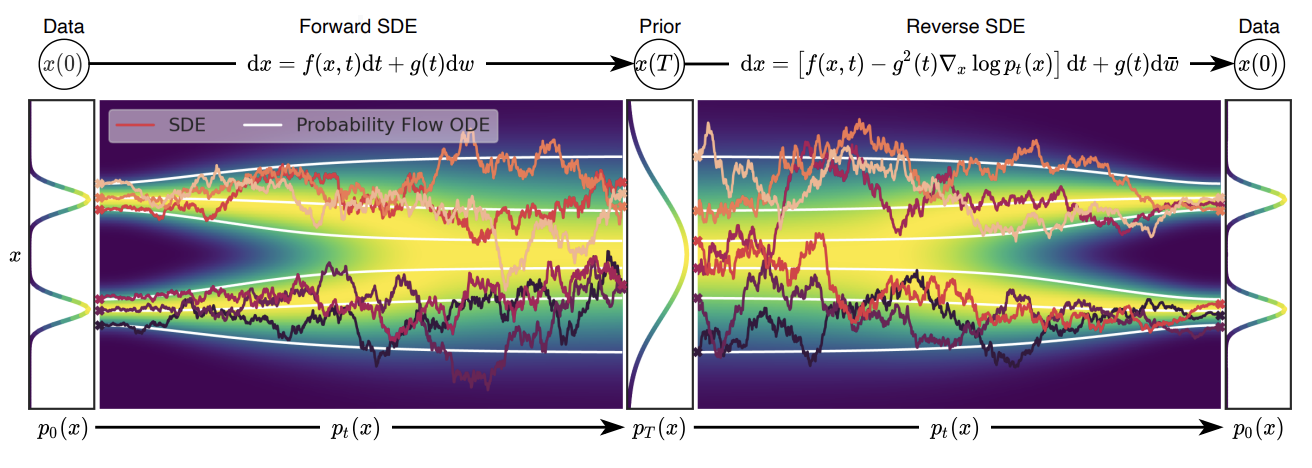
\includegraphics[width=0.8\textwidth]{Figures/diffusion.png}
    \caption{Forward and Backward Processes in Diffusion Models (The picture is from Song and Ermon (2019))}
    \label{fig:forward-backward}
\end{figure}

\section{VE, VP SDEs}

\subsection{Continuos Forward Process}
After we established the general form of the forward and backward processes, we can now go back to see how to apply them on SMLD (VE mthoed) and DDPM (VP method).

So in this section, we try to present detailed derivations demonstrating that the noise perturbations in SMLD (Score-based generative modeling via Langevin Dynamics) and DDPM (Denoising Diffusion Probabilistic Models) are discretizations of the Variance Exploding (VE) and Variance Preserving (VP) Stochastic Differential Equations (SDEs), respectively. 

First, when utilizing a total of \( N \) noise scales, each perturbation kernel \( p_{\sigma_i}(x | x_0) \) for SMLD can be derived from the following Markov chain:

\begin{equation}
x_i = x_{i-1} + \sqrt{\sigma_i^2 - \sigma_{i-1}^2} z_{i-1}, \quad i = 1, 2, \ldots, N,
\end{equation}

\noindent
where \( z_{i-1} \sim \mathcal{N}(0, I) \) and \( x_0 \sim p_{\text{data}} \). Here, we introduce \( \sigma_0 = 0 \) for simplicity. As \( N \to \infty \), the Markov chain \( \{ x_i \}_{i=1}^N \) converges to a continuous stochastic process \( \{ x(t) \}_{t=0}^1 \), and \( \{ \sigma_i \}_{i=1}^N \) becomes a function \( \sigma(t) \), while \( z_i \) transitions to \( z(t) \). We denote the continuous time variable as \( t \in [0, 1] \) instead of the integer index \( i \in \{ 1, 2, \ldots, N \} \). Let $\mathbf{x} ( \frac{i}{N} ) = \mathbf{x}_i$, $\mathbf{\sigma} ( \frac{i}{N} ) = \mathbf{\sigma}_i$, $\mathbf{z} ( \frac{i}{N} ) = \mathbf{z}_i$, for $i = 1, 2, \ldots, N$. 
Rewriting Equation \refeq{eq:ddpm-discrete} with $\Delta t = \frac{1}{N}$ gives:
 
\begin{equation}
x(t + \Delta t) = x(t) + \sqrt{\sigma^2(t + \Delta t) - \sigma^2(t)} z(t) \approx x(t) + \sqrt{\frac{d \sigma^2(t)}{dt}} \Delta t z(t),
\end{equation}

\noindent
where the approximation holds as \( \Delta t \to 0 \). In the limit of \( \Delta t \to 0 \), we obtain the VE SDE:

\begin{equation}
dx = \sqrt{\frac{d \sigma^2(t)}{dt}} dw.
\end{equation}

\noindent
Furthermore, we usually let $\sigma$ sequence to be a geometric sequence. We have $\sigma (\frac{i}{N}) = \sigma_i = \sigma_{\min} (\frac{\sigma_{\max}}{\sigma_{\min}})^{\frac{i-1}{N-1}}$ for i ranges from 1 to N. If \( N \to \infty \)

\noindent
The corresponding VE SDE is 

\begin{equation}
    d \mathbf{x} = \sigma_{\min} \left( \frac{\sigma_{\max}}{\sigma_{\min}} \right) ^t \sqrt{2 \log \left( \frac{\sigma_{\max}}{\sigma_{\min}} \right) } \, d \mathbf{w}, \quad t \in (0, 1).
\end{equation}

\noindent
For the perturbation kernels \( p_{\alpha_i}(x | x_0) \) used in DDPM, the discrete Markov chain is given by:

\begin{equation}
\mathbf{x}_i = \sqrt{1 - \beta_i} \mathbf{x}_{i-1} + \sqrt{1 - \beta_i} z_{i-1}, \quad i = 1, 2, \ldots, N \label{eq:ddpm-discrete}
\end{equation}

\noindent
where \( z_{i-1} \sim \mathcal{N}(0, I) \). To obtain the limit of this Markov chain as \( N \to \infty \), we define an auxiliary set of noise scales \( \{ \bar{\beta}_i \}_{i=1}^N \) and rewrite Equation \refeq{eq:ddpm-discrete} as follows:

\begin{equation}
\mathbf{x}_i = \sqrt{1 - \bar{\beta}_i} \mathbf{x}_{i-1} + \sqrt{1 - \bar{\beta}_i} z_{i-1}, \quad i = 1, 2, \ldots, N \label{eq:ddpm-discrete}
\end{equation}

\noindent
As \( N \to \infty \), the noise scales \( \{ \bar{\beta}_i \}_{i=1}^N \) converge to a function \( \beta(t) \) indexed by \( t \in [0, 1] \). Let \( \{ \bar{\beta}_i \}_{N} = \beta \) and \( \{ x_i \}_{N} = x \) and \( \{ z_i \}_{N} = z \). Rewriting Equation \refeq{eq:vp-sde} gives:

\begin{equation}
\begin{aligned}
    \mathbf{x}(t + \Delta t) &= \sqrt{1 - \beta(t + \Delta t)} \mathbf{x}(t) + \sqrt{1 - \beta(t + \Delta t)} z(t) \\ &\approx \mathbf{x}(t) -\frac{1}{2}\beta(t + \Delta t) \Delta t \mathbf{x}(t)+\sqrt{\beta(t + \Delta t) \Delta t } \mathbf{z} (t) \\
    &\approx \mathbf{x}(t) -\frac{1}{2}\beta(t ) \Delta t \mathbf{x}(t)+\sqrt{\beta(t ) \Delta t } \mathbf{z} (t) 
\end{aligned} \label{eq:ddpm-discrete}
\end{equation}

\noindent
where the approximation holds as \( \Delta t \to 0 \). Therefore, in the limit of \( \Delta t \to 0 \), we obtain the VP SDE:

\begin{equation}
d \mathbf{x} = -\frac{1}{2} \beta(t) \mathbf{x} \, dt + \sqrt{\beta(t)} \, d\mathbf{w}.\label{eq:vp-sde}
\end{equation}

\noindent
As in DDPM, $\beta$ is typically an arithmetic sequence where $\beta_i = \beta_{\min} + t (\beta_{\max} - \beta_{\min}) $ for t ranges from 0 to 1 if \( N \to \infty \). This will then give us the VP SDE as

\begin{equation}
    d \mathbf{x} = -\frac{1}{2} \left( \beta_{\min} + t (\beta_{\max} - \beta_{\min} )\right) \mathbf{x} \, dt + \sqrt{\beta_{\min} + t (\beta_{\max} - \beta_{\min})} \, d\mathbf{w}, \quad t \in (0, 1).
\end{equation}

\noindent
In conclusion, the contents above indicate that 

\noindent
For SMLD (Variance Exploding SDE - VE):
\begin{itemize}
    \item \( f(x, t) = 0 \)
    \item \( g(t) = \sigma_{\min} \left( \frac{\sigma_{\max}}{\sigma_{\min}} \right)^t \sqrt{2 \log \left( \frac{\sigma_{\max}}{\sigma_{\min}} \right)} \)
\end{itemize}

\vspace{1em}

\noindent
For DDPM (Variance Preserving SDE - VP):
\begin{itemize}
    \item \( f(x, t) = -\frac{1}{2} \beta(t) x \)
    \item \( g(t) = \sqrt{\beta(t)} \)
\end{itemize}

\subsection{Continuos Backward Process - PC Sampler}

Here we can of course use the $f(x,t)$ and $g(t)$ to do the reverse process as equation \eqref{eq:reverse} shows. However, here we possess additional insights that can enhance our solution methods. Specifically, with our score-based model 
$s_{\theta^*}(x, t) \approx \nabla_x \log p_t(x)
$, we can utilize score-based Markov Chain Monte Carlo (MCMC) techniques to sample directly from the distribution $p_t$ and refine the outputs of a numerical SDE solver.

At each time step, the numerical SDE solver provides an initial estimate for the sample at the next time step, functioning as a "predictor." Subsequently, the score-based MCMC method adjusts the estimated sample's marginal distribution, acting as a "corrector." This approach is reminiscent of Predictor-Corrector methods. We similarly refer to our hybrid sampling algorithms as Predictor-Corrector (PC) samplers.

The PC samplers extend the original sampling methodologies of SMLD and DDPM: the SMLD method employs an identity function as the predictor and utilizes annealed Langevin dynamics as the corrector. In contrast, the DDPM method adopts ancestral sampling as the predictor and the identity function as the corrector.

\noindent\textbf{Algorithm 1} \textit{PC sampling (VE SDE)}
\begin{algorithmic}[1]
    \STATE $\mathbf{x}_N \sim \mathcal{N}(0, \sigma_{\max}^2 \mathbf{I})$
    \FOR{$i = N - 1$ to $0$}
        \STATE $\mathbf{x}'_i = \mathbf{x}_i -g^2(t)s_\theta^* \left( \mathbf{x}_i, \sigma_i \right) {\Delta t}$
        \STATE $\mathbf{z} \sim \mathcal{N}(0, \mathbf{I})$
        \STATE $\mathbf{x}_i = \mathbf{x}'_i +g(t) \sqrt{\Delta t} \mathbf{z}$
        \FOR{$j = 1$ to $M$}
            \STATE $\mathbf{z} \sim \mathcal{N}(0, \mathbf{I})$
            \STATE $\mathbf{x}_i \leftarrow \mathbf{x}_i + \epsilon_i s_\theta^* \left( \mathbf{x}_i, \sigma_i \right) + \sqrt{2 \epsilon_i} \mathbf{z}$
        \ENDFOR
    \ENDFOR
    \RETURN $\mathbf{x}_0$
\end{algorithmic}

\bigskip

\noindent\textbf{Algorithm 2} \textit{PC sampling (VP SDE)}
\begin{algorithmic}[1]
    \STATE $\mathbf{x}_N \sim \mathcal{N}(0, \mathbf{I})$
    \FOR{$i = N - 1$ to $0$}
        \STATE $\mathbf{x}'_i = (f(x,t)-g^2(t)*s_\theta^* \left( \mathbf{x}_{i+1}, i+1 \right)) {\Delta t}$
        \STATE $\mathbf{z} \sim \mathcal{N}(0, \mathbf{I})$
        \STATE $\mathbf{x}_i = \mathbf{x}'_i +g(t) \sqrt{\Delta t} \mathbf{z}$
        \FOR{$j = 1$ to $M$}
            \STATE $\mathbf{z} \sim \mathcal{N}(0, \mathbf{I})$
            \STATE $\mathbf{x}_i \leftarrow \mathbf{x}_i + \epsilon_i s_\theta^* \left( \mathbf{x}_i, i \right) + \sqrt{2 \epsilon_i} \mathbf{z}$
        \ENDFOR
    \ENDFOR
    \RETURN $\mathbf{x}_0$
\end{algorithmic}

where $\epsilon$ is defined as 

\begin{equation}
    \epsilon = 2 r^2 \frac{\|\mathbf{z}\|_2^2}{\|s_\theta\|_2^2}
\end{equation}

and $r$ is a hyperparameter that controls the step size of the Langevin dynamics.







